\section{Digrafos}


Los \emph{grafos dirigidos} o \emph{digrafos} son grafos en los que las aristas tienen una direcci\'on.


\subsection{Grafos dirigidos}


Un grafo dirigido $G=G(V,E)$ consiste de:
\begin{enumerate}
	\item Un conjunto $V=V(G)$ cuyos elementos son llamados \emph{v\'ertices};
	\item un conjunto $E=E(G)$ de \emph{pares ordenados} ordenados de v\'ertices llamados \emph{arcos} o \emph{aristas dirigidas.}
\end{enumerate}




Supongamos que $e=(u,v)$ es un arco en el digrafo $G.$ Entonces, la siguiente terminolog\'ia es usada:
\begin{itemize}
	\item $e$ comienza en $v$ y termina en $v;$
	\item $u$ es el origen o punto inicial de $e,$ mientras que $v$ es el destino o punto final de $e.$
	\item $v$ es un sucesor de $u;$
	\item $u$ es adyacente a $v$ y $v$ es adyacente desde $u.$
\end{itemize}


Si $u=v,$ $e$ es llamado un \emph{bucle.}



Si las aristas o los v\'ertices de un digrafo est\'an etiquetas con alg\'un tipo de dato, diremos que es un \emph{digrafo etiquetado.}


De manera similar a un grafo, un digrafo ser\'a finito si el conjunto de v\'ertices y el de aristas es finito.



\begin{exmp}
	Consideremos el siguiente digrafo.
	\begin{figure}[h]
		\centering
		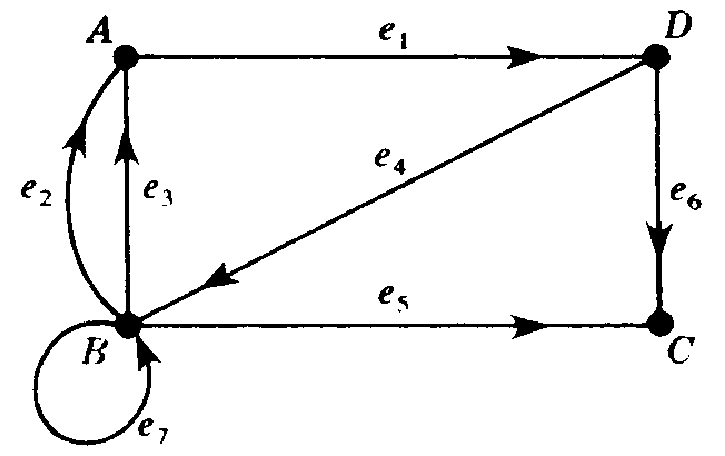
\includegraphics[height=3cm,keepaspectratio=true]{./md/fig0901a.png}
		% fig0901a.png: 0x0 pixel, 300dpi, 0.00x0.00 cm, bb=
		%\caption{Digrafo}
		\label{fig:0901a}
	\end{figure}
	Las aristas $e_{2}$ y $e_{3}$ son llamados \emph{paralelos,} ya que ambos comienzan en $B$ y terminan en $A.$ La arista $e_{7}$ es un \emph{bucle.}
\end{exmp}




\begin{exmp}
	\begin{figure}[h]
		\centering
		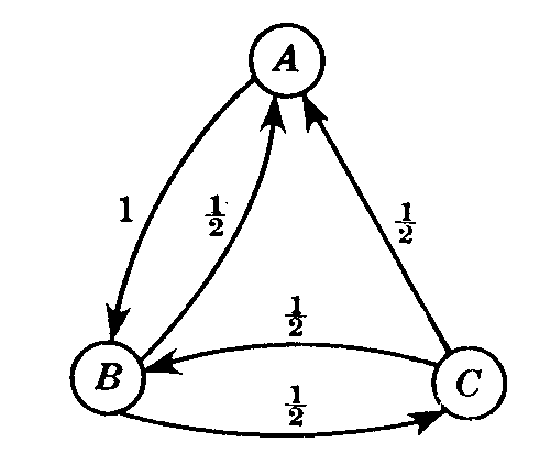
\includegraphics[width=5cm,keepaspectratio=true]{./md/fig0901b.png}
		% fig0901b.png: 0x0 pixel, 300dpi, 0.00x0.00 cm, bb=
		\caption{Proceso estocástico}
		\label{fig:0901b}
	\end{figure}
	
\end{exmp}



\subsection{Matriz de adyacencia}


Ahora, s\'olo consideraremos \emph{digrafos simples} $G(V,E)$, es decir, sin aristas paralelas. Entonces $E$ es simplemente una relaci\'on en $V.$ 

De manera inversa, si $R$ es una relaci\'on en $V,$ entonces $G(V,R)$ es un digrafo simple.

En unidades anteriores, ya hemos construido digrafos asociados a relaciones de orden parcial, llamados diagramas de Hasse. 



Supongamos que $G$ es un digrafo simple con $m$ v\'ertices, y supongamos que los v\'ertices de $G$ han sido ordenados y son llamados $v_{1}, v_{2},...,v_{m}.$ 

Entonces la \emph{matrix de adyacencia} $A=\left( a_{i,j} \right)$ de $G$ es la una matriz de dimensi\'on $m\times m$ definida de la siguiente manera
$$a_{i,j}=
\begin{cases}
	1 & \exists e \in E: e=(v_{i}, v_{j})\\
	0 & \texttt{en otro caso}
\end{cases}
$$



\begin{rem}
	Las matrices de adyacencia de un mismo grafo dependen del orden en que se enumeren los v\'ertices. 
	Sin embargo, dos matrices de adyacencia de un mismo grafo est\'an relacionadas por operaciones elementales: cambiar el orden de columnas y renglones. 
\end{rem}




\begin{exmp}
	Sea $G$ el siguiente digrafo
	\begin{figure}[h]
		\centering
		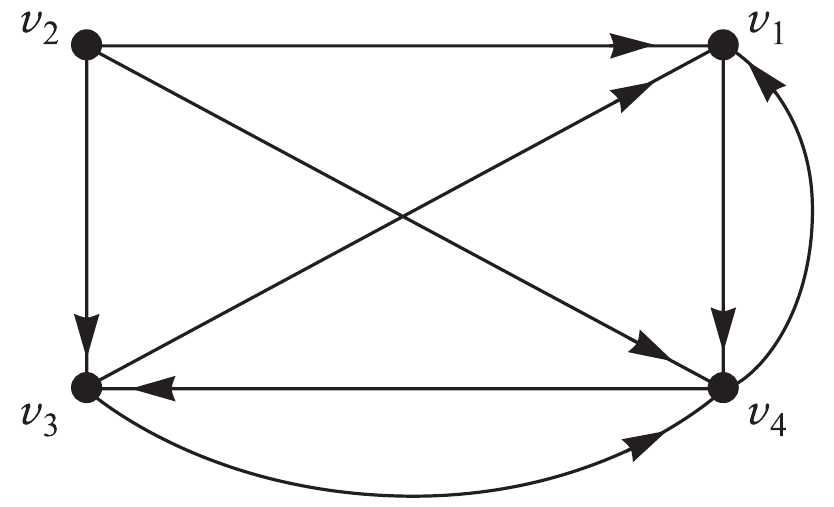
\includegraphics[height=3cm,keepaspectratio=true]{./md/fig0904a.png}
		% fig0904a.png: 0x0 pixel, 300dpi, 0.00x0.00 cm, bb=
		\caption{Construya su matriz de adyacencia del digrado anterior.}
		\label{fig:0904a}
	\end{figure}
	
\end{exmp}




La matriz identidad $I_{m}=\left( I_{i,j} \right)$ de dimensi\'on $m\times m$ se define como
$$I_{i,j}
\begin{cases}
	1 & i=j \\
	0 & i \neq j,
\end{cases}
$$
es decir, es matriz cuadrangular con $1's$ en la \emph{diagonal principal}, y ceros en cualquier otra entrada.



\begin{exmp}
	$$I_{2}=
	\begin{pmatrix}
		1 & 0 \\
		0 & 1 \\
	\end{pmatrix}
	$$
	
	$$I_{3}=
	\begin{pmatrix}
		1 & 0 & 0 \\
		0 & 1 & 0 \\
		0 & 0 & 1
	\end{pmatrix}
	$$
\end{exmp}




La propiedad principal de una matriz identidad $I_{m}$ es que es nuestra respecto a la multiplicaci\'on de matrices, es decir, para cualquier otra matriz $A\in M_{n}:$
$$
AI_{n}=I_{n}A=A.
$$



La potencia $n-$\'esima de una matriz $A \in M_{n}$ se define de manera recursiva como
$$
A^{n}=
\begin{cases}
	I_{n}  & n=0\\
	AA^{n-1} & n \in \N.
\end{cases}
$$ 

Es decir, $$A^{0}=I, A^{1}=A, A^{2}=AA,...$$



Definamos $a_{k}(i,j)$ como la entrada en la posici\'on $i,j$ de $A^{k}.$


\begin{prop}
	Sea $A$ la matriz de adyacencia de un grafo $G.$ Entonces $a_{k}(i,j)$ es igual al n\'umero de caminos de longitud $k$ que van de $v_{i}$ a $v_{j}.$
\end{prop}



{Ejemplo}
Consideremos nuevamente el grafo
\begin{figure}[h]
	\centering
	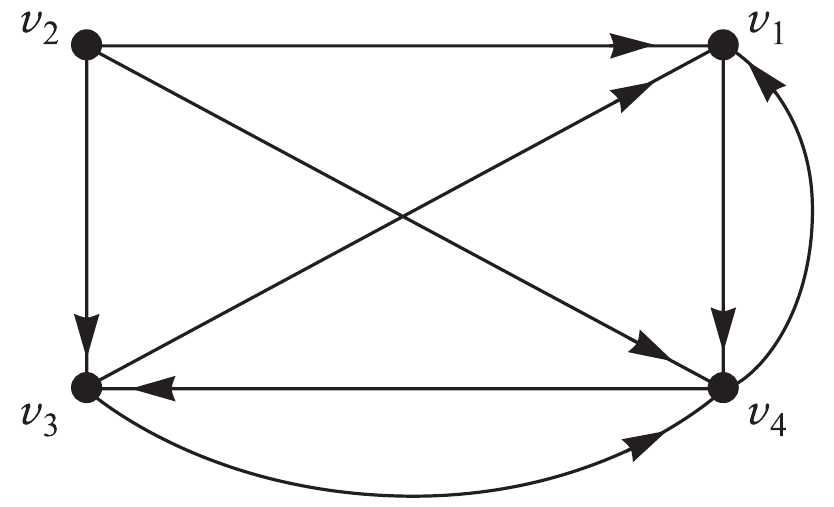
\includegraphics[height=3cm,keepaspectratio=true]{./md/fig0904a.png}
	% fig0904a.png: 0x0 pixel, 300dpi, 0.00x0.00 cm, bb=
\end{figure}



Recordemos que su matriz de adyacencia es
\begin{equation}
	\label{exmp:adj}
	\tag{AD}
	A= \left(\begin{array}{rrrr}
		0 & 0 & 0 & 1 \\
		1 & 0 & 1 & 1 \\
		1 & 0 & 0 & 1 \\
		1 & 0 & 1 & 0
	\end{array}\right)
\end{equation}




Entonces
$$
A^{2}= \left(\begin{array}{rrrr}
	1 & 0 & 1 & 0 \\
	2 & 0 & 1 & 2 \\
	1 & 0 & 1 & 1 \\
	1 & 0 & 0 & 2
\end{array}\right) \;
A^{3}= \left(\begin{array}{rrrr}
	1 & 0 & 0 & 2 \\
	3 & 0 & 2 & 3 \\
	2 & 0 & 1 & 2 \\
	2 & 0 & 2 & 1
\end{array}\right) \;
$$

$$
A^{4}= \left(\begin{array}{rrrr}
	2 & 0 & 2 & 1 \\
	5 & 0 & 3 & 5 \\
	3 & 0 & 2 & 3 \\
	3 & 0 & 1 & 4
\end{array}\right)
$$



Observe que $a_{2}(4,1)=1,$ de manera que existe un solo camino de longitud 2 de $v_{4}$ a $v_{1}.$ De manera similar, como $a_{3}(2,3)=2,$ entonces existen dos caminos de longitud $3$ de $v_{2}$ a $v_{3}.$



\begin{rem}
	Si definimos 
	$$B_{r}= \sum_{i=1}^{r}A^{i},$$
	entonces la entrada $i,j$ de esta matriz nos indicar\'a el n\'umero de caminos de longitud a lo m\'as $r$ de $v_{i}$ a $v_{j}.$
\end{rem}



En nuestro ejemplo, considerando $A$ dado por \eqref{exmp:adj}, tenemos que 
\begin{equation}
	\label{B4}
	B_{4}=
	\left(\begin{array}{rrrr}
		4 & 0 & 3 & 4 \\
		11 & 0 & 7 & 11 \\
		7 & 0 & 4 & 7 \\
		7 & 0 & 4 & 7
	\end{array}\right)
\end{equation}


?`Existe alguna manera de llegar al vertice $v_{2}$ desde el v\'ertice $v_{1}$, sin importar la longitud del camino?


\subsection{Matriz de accesibilidad}


Sea $G=G(V,E)$ un grafo simple dirigido con $m$ v\'ertices $v_{1},...,v_{m}.$ La \emph{matriz de accesibilidad} de $G$ es la matriz $m-$cuadrangular $P=\left( p_{ij} \right)$ definida de la siguiente manera:
$$p_{ij}=
\begin{cases}
	1 & \texttt{existe un camino de }v_{i}\texttt{ a }v_{j}\\
	0 & \texttt{en otro caso}
\end{cases}
$$



\begin{prop}
	Sea $A$ la matriz de adyacencia de un grafo $G$ con $m$ v\'ertices. Entonces la matriz de accesibilidad y 
	\begin{equation}
		\label{Bm}
		B_{m}=\sum_{i=1}^{m}A^{i}
	\end{equation}
	tienen exactamente las mismas entradas no nulas. 
\end{prop}




\begin{defn}
	Un digrafo es \emph{fuertemente conexo} si para cualquier par de v\'ertices $u,v$ existe al menos un camino de $u$ a $v$ y otro de $v$ a $u.$
\end{defn}




\begin{prop}
	Sea $A\in M_{m}$ la matriz de adyacencia de un grafo $G.$ Entonces, las siguientes proposiciones son equivalentes:
	\begin{enumerate}
		\item $G$ es fuertemente conexo;
		\item la matriz de accesibilidad $P$ no tiene entradas nulas;
		\item la matriz $B_{m},$ dada por \eqref{Bm}, no tiene entradas nulas.
	\end{enumerate}
	
\end{prop}




\begin{exmp}
	\label{lip:exmp:0908}
	Para encontrar la matriz de accesibilidad asociada a la matriz de adyacencia $A,$ dada por \eqref{exmp:adj}, basta sustitur las entradas no nulas en la matriz $B_{4},$ dada por \eqref{B4}, por $1's:$
	$$
	P=
	\left(\begin{array}{rrrr}
		1 & 0 & 1 & 1 \\
		1 & 0 & 1 & 1 \\
		1 & 0 & 1 & 1 \\
		1 & 0 & 1 & 1
	\end{array}\right)
	$$
\end{exmp}


